\documentclass[12pt,convert={false}]{standalone}
\usepackage[dvipsnames]{xcolor}
\usepackage{tikz}
\usetikzlibrary{shapes,arrows,positioning,calc,patterns,arrows.meta, bending, graphs, shadings,quotes,intersections}
\usetikzlibrary{external}
%\tikzexternalize[prefix=tikz/]
\usepackage{pgfplots}
\pgfplotsset{compat=1.16}
\usepgfplotslibrary{fillbetween}
\newcommand{\enf}[1]{\textcolor{RedViolet}{\textbf{#1}}} %enf sta per enfasi
\newcommand{\sott}[1]{\setulcolor{black!20!Goldenrod}\ul{#1}}
\newcommand{\prob}{\mathbb{P}}
\newcommand\independent{\protect\mathpalette{\protect\independenT}{\perp}}
\newcommand{\ev}[1]{\mathbb{E}\Bigl[{#1}\Bigr]}
\def\independenT#1#2{\mathrel{\rlap{$#1#2$}\mkern2mu{#1#2}}}
\newcommand{\Z}{\mathbb{Z}}
\newcommand{\R}{\mathbb{R}}
\newcommand{\N}{\mathbb{N}}
\newcommand{\equalexpl}[1]{%
	\underset{\substack{\uparrow\\\mathrlap{\text{\vspace{-3cm}\hspace{-1em}#1}}}}{=}}
\newcommand{\dif}{\mathop{}\!\mathrm{d}}
\begin{document}
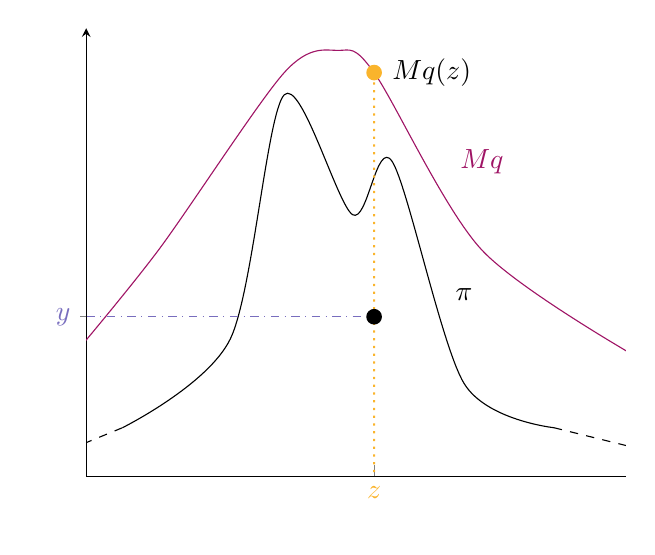
\begin{tikzpicture}%[scale=0.8]
	\begin{axis}[
		xlabel=\empty,
		x axis line style={opacity=100},
		ylabel=\empty,
		xmin=-1, xmax=1500,
		ymin=-1, ymax=100,
		axis y line=left,
		y axis line style={opacity=100},
		ytick={35},
		xtick={800},
		xticklabels={\textcolor{Dandelion}{$z$}},
		yticklabels={\textcolor{Periwinkle}{$y$}},
		axis x line*=bottom
		]
		\addplot[smooth,restrict x to domain=50:1300] coordinates {
			(100,10)
			(400,30)
			(550,85)
			(740,58)
			(850,70)
			(1050,20)
			(1300,10)
		};
		\addplot[smooth,dashed,restrict expr to domain={(x>=-50)&&(x<=100)||(x>=1300)&&(x<=1550)}{1:1}] coordinates {
			(-50,5)
			(100,10)
			(400,30)
			(550,85)
			(740,58)
			(850,70)
			(1050,20)
			(1300,10)
			(1550,5)
		};
		\addplot[smooth, RedViolet, name path=M] coordinates {
			(-50,25)
			(200,50)
			(550,90)
			(700,95)
			(800,90)
			(1100,50)
			(1550,25)
		};
		\node[align=left] at (1050,40) {$\pi$};
		\node[align=left,RedViolet] at (1100,70) {$Mq$};
		\path [name path=A] (axis cs: 800, 0) -- (axis cs: 800, 100);
		\path [name intersections={of=A and M}];
		\draw [dotted, thick, Dandelion] (800,0) -- (intersection-1);
		\node [circle,Dandelion,fill,inner sep=2pt,label=right:{$Mq(z)$}] at (intersection-1) {};
		\draw [dash dot,Periwinkle] (0,35)--(800,35);
		\node [circle,fill,inner sep=2pt] at (800,35) {};
	\end{axis}
\end{tikzpicture}
\end{document}
